\documentclass[conference]{IEEEtran}

% --- Packages ---
\usepackage{graphicx}
\usepackage{booktabs}
\usepackage{amsmath,amssymb}
\usepackage{siunitx}
\usepackage[caption=false,font=footnotesize]{subfig} % instead of caption
\usepackage{url} % for \url{...}
\usepackage[hidelinks]{hyperref} % keep last

% Optional hyphenation help
\hyphenation{mi-cros-copy neu-ro-im-ag-ing flu-o-res-cence ras-ter two-pho-ton}


% --- Title & Authors ---
\title{NAOMi: End-to-End Simulation of Two-Photon Calcium Imaging\\with an Integrated Overview and Demonstration}

\author{\IEEEauthorblockN{Jaeho Cho}
\IEEEauthorblockA{The Cooper Union\\New York, NY, USA\\Email: jaeho.cho@cooper.edu}}

\begin{document}
\maketitle

\begin{abstract}
The Neural Anatomy and Optical Microscopy (NAOMi) simulator generates realistic, ground-truth two-photon calcium-imaging datasets by modeling neural anatomy, activity-dependent fluorescence, optical propagation, raster scanning, motion, and detector noise. This paper presents a concise demonstration run for readers with electrical and bioengineering backgrounds and provides an integrated, expanded overview of the original NAOMi work, including design goals, architecture, validation against in~vivo data, algorithm benchmarking, optical-design studies, availability/performance, and limitations. We also note a contemporary use case (NORA) where NAOMi serves as a testbed for acquisition--reconstruction co-design. Static mean/max projections are shown, and supplementary videos more clearly illustrate the contrast between noisy and clean renderings.
\end{abstract}

\begin{IEEEkeywords}
Two-photon microscopy, calcium imaging, computational imaging, neuroscience
\end{IEEEkeywords}

\section{Introduction}
Two-photon microscopy enables cellular-resolution recordings across neuronal populations. Yet tuning optical parameters and benchmarking analysis pipelines are challenging without access to ground truth. NAOMi provides a controllable, biophysically motivated simulator that outputs videos resembling in~vivo recordings while retaining latent truth (anatomy and activity). This enables systematic studies of trade-offs among spatial resolution, frame rate, field of view, depth, and noise, and supports repeatable evaluation of segmentation, denoising, demixing, and inference methods.

\section{Overview of NAOMi}\label{sec:overview}
\subsection{Design Goals and Scope}
NAOMi was designed as a fast, end-to-end simulator producing realistic two-photon datasets with known ground truth, enabling fair and repeatable comparisons of optical designs and analysis algorithms. The scope spans 3-D neuroanatomy synthesis, activity-dependent fluorescence, depth-aware optical propagation, raster scanning, motion, and detection noise (photon shot noise with optional read/amplifier noise). The original study validated NAOMi by matching simulated statistics to in~vivo recordings and by comparing common segmentation methods and specialized optical setups.

\subsection{System Architecture}
The simulator comprises four coupled modules:
\begin{enumerate}
  \item \textbf{Neural volume generation.} A cortical volume is populated with vasculature, somata, and neurites (dendrites/axons). The output stores locations and fluorophore densities for cells, neurites, and background.
  \item \textbf{Activity to fluorescence.} Neuronal spike trains are simulated and mapped to calcium and bound-calcium concentrations, then to fluorescence via an indicator model. For speed, a short-memory (AR-like) filter approximates kinetics, yielding smooth $\Delta F/F$ traces with controllable time constants and amplitudes. Spatial proximity can induce mild correlations among nearby elements.
  \item \textbf{Optical propagation and PSF.} An optical wavefront (set by the microscope) is propagated through a scattering volume to produce a depth-varying point-spread function (PSF) and an optical mask accounting for attenuation and warping from tissue and vasculature; this modulates local excitation/collection efficiency.
  \item \textbf{Scanning, motion, and detection.} A raster scanner integrates PSF-weighted fluorescence along fast/slow axes; optional rigid/nonrigid motion and detection noise are injected through a light-collection/amplification/digitization model. The output includes a noisy movie and a motion-consistent clean companion movie without detection noise.
\end{enumerate}

\subsection{Validation Against In~Vivo Data}
Simulations were compared to mouse visual cortex recordings expressing GCaMP, with agreement across: (i) mean images and pixel-value distributions; (ii) distributions of maximum $\Delta F/F$ across pixels; (iii) spatial frequency content influenced by line scanning, motion, and pixel bleed-through; and (iv) low-rank structure (PCA variance decay and spatial PCs). These results support realism in spatial and temporal statistics.

\subsection{Algorithm Benchmarking on Ground Truth}
Using NAOMi data with known spatial profiles and time courses, common segmentation pipelines (e.g., CNMF, Suite2p, PCA/ICA) were compared against oracle-assisted baselines. Strong neural time courses were recovered with correlations near those obtained using oracle spatial information, though with elevated false-positive rates---quantifiable via ROC analysis, correlation thresholds, footprint overlap, and spike-timing metrics. NAOMi thus enables principled measurement of trade-offs.

\subsection{Optical-Design Studies}
NAOMi was used to compare specialized modalities against a standard high-NA Gaussian two-photon setup under varying labeling densities and volumetric schemes. Representative findings include: (i) Bessel beams improving resilience to motion artifacts under sparse labeling; (ii) lower-NA Gaussian excitation plus nuclear GCaMP increasing SNR and the number of extractable cells in nuclear-labeled samples; and (iii) temporal focusing providing more uniform spatial sampling than certain multi-plane configurations during volumetric imaging. These studies illustrate optics--algorithm co-design under controlled conditions.

\subsection{Limitations and Intended Use}
For tractability, NAOMi simplifies several phenomena: tissue scattering and motion are approximated; photobleaching/photodamage and hemodynamics are simplified; and sensor electronics are captured at a lumped level. The framework targets relative comparisons and ablation studies (e.g., how SNR or segmentation accuracy changes with NA, dwell time, depth, labeling, or noise) rather than exact replication of a specific experiment.

\section{Simulation Demonstration}\label{sec:methods}
A standard pipeline was executed to produce representative movies. The steps mirror the public NAOMi code:
\begin{enumerate}
  \item \textbf{Scene generation:} \texttt{simulate\_neural\_volume} builds the 3-D volume with neural and vascular elements.
  \item \textbf{Optics:} \texttt{simulate\_optical\_propagation} computes a depth-varying PSF and mask.
  \item \textbf{Activity:} \texttt{generateTimeTraces} produces per-element fluorescence time courses.
  \item \textbf{Scanning:} \texttt{scan\_volume} outputs the noisy movie \texttt{Fsim} and the clean movie \texttt{Fsim\_clean}.
\end{enumerate}
Principal settings are summarized in Table~\ref{tab:params}.

\begin{table}[t]
\centering
\caption{Principal simulation settings for the demonstration.}
\label{tab:params}
\begin{tabular}{@{}ll@{}}
\toprule
\textbf{Volume size} & $100\times100\times100\,\mu\text{m}$ \\
\textbf{Imaging depth (center)} & $100\,\mu\text{m}$ \\
\textbf{Objective NA} & 0.8 \\
\textbf{Excitation (beam) NA} & 0.6 \\
\textbf{Average power} & \SI{40}{\milli\watt} \\
\textbf{Frames and rate} & 2{,}500 at 30\,Hz ($\Delta t = 1/30$\,s) \\
\textbf{Mean event rate} & $\approx 0.25$ per component per second \\
\textbf{Motion} & Off (toggle available) \\
\textbf{Noise model} & Photon shot noise with optional read noise \\
\bottomrule
\end{tabular}
\end{table}

\section{Results}\label{sec:results}
Figure~\ref{fig:meanmax} shows mean and maximum-intensity projections derived
from the simulated movies.

Although both noisy and clean movies are generated, the static mean/max
projections appear almost identical. This is expected under the chosen
demonstration settings: 2{,}500 frames at 30\,Hz with motion disabled and
high average power (\SI{40}{\milli\watt}) produce high photon counts with
noise that is largely zero-mean across time. In the mean projection, random
fluctuations cancel as $1/\sqrt{N}$ ($N$ frames), driving the noisy mean
toward the clean mean. In the maximum projection, true neuronal structures
dominate the peak intensity across frames, so occasional noise spikes do
not strongly alter the outcome at this signal-to-noise ratio. By contrast,
the videos make the difference more apparent, since frame-
to-frame fluctuations are preserved there.

% Two-column wide figure for the embedded PDF
\begin{figure*}[t]
  \centering
  % Place meanAndMaxImages.pdf alongside this .tex file when compiling.
  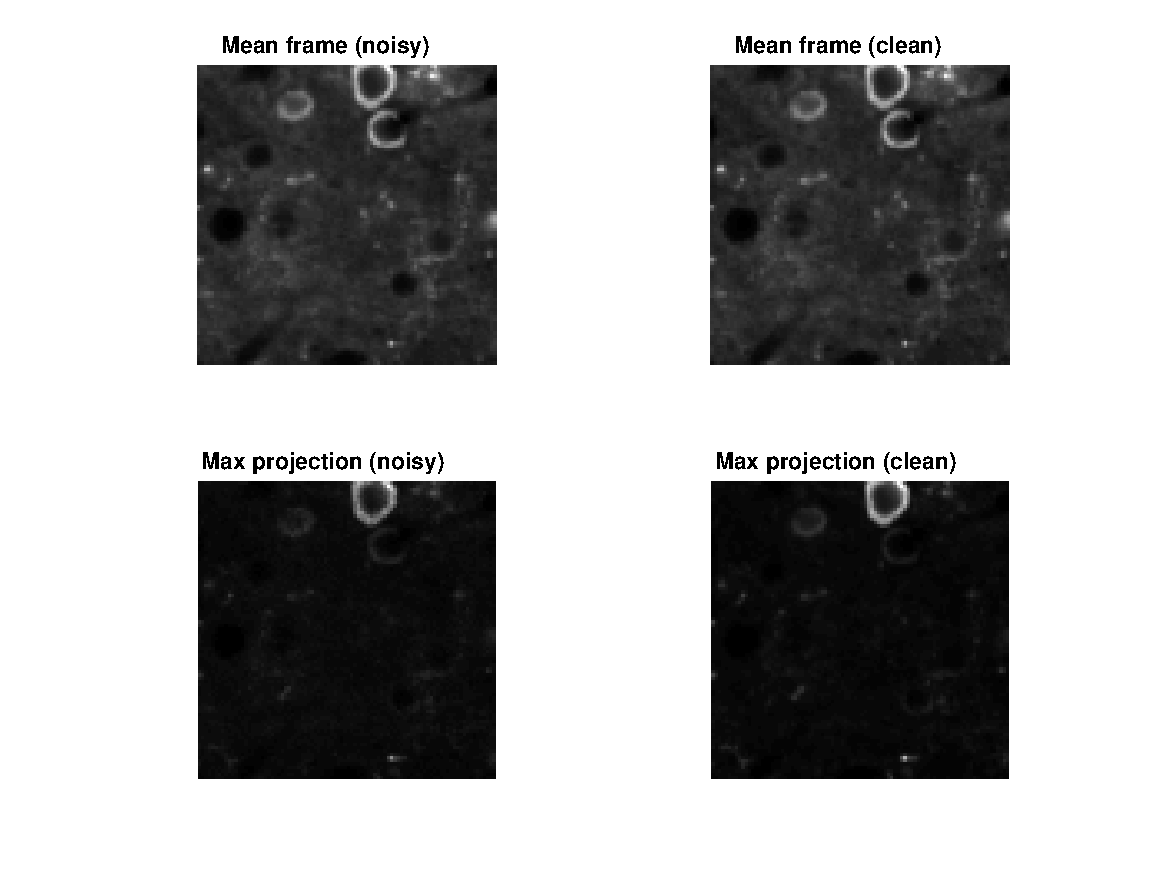
\includegraphics[width=0.98\textwidth]{meanAndMaxImages.pdf}
  \caption{Mean and maximum intensity projections from the simulated dataset. The dynamic difference between noisy and clean is clearer when viewing the videos.}
  \label{fig:meanmax}
\end{figure*}

\section{Contemporary Use: NORA}\label{sec:nora}
Cooper Alumni, Esther Whang EE'23, developed NORA (Neuroimaging with Oblong Random Acquisition) to reduce per-frame sampling while preserving information needed for later recovery. Practically, NORA subsamples scan lines and adjusts the effective PSF to collect signal across neighboring lines, then reconstructs the full video jointly using a low-rank prior. NAOMi provides realistic benchmark movies with known ground truth and controllable noise/motion, enabling systematic evaluation across sampling factors, SNR levels, and motion settings.

\section{Discussion}\label{sec:discussion}
NAOMi offers a practical means to explore design choices in two-photon imaging prior to hardware changes or animal experiments:
\begin{itemize}
  \item \textbf{Design exploration:} Sweep NA, laser power, depth, dwell time, and noise to study resolution--throughput--SNR trade-offs.
  \item \textbf{Algorithm evaluation:} Use ground-truth footprints and time courses to quantify segmentation accuracy, trace fidelity, and event timing.
  \item \textbf{Shared framework:} A common simulator aligns optical, computational, and biological considerations.
\end{itemize}
Limitations include simplified scattering and motion models and approximate fluorescence kinetics, but the framework is sufficient for comparative studies and method development.

\section{Conclusion}\label{sec:conclusion}
NAOMi enables end-to-end, reproducible simulations of two-photon calcium imaging with access to ground truth. The demonstration follows a standard pipeline and illustrates how static projections and companion videos capture the effect of detection noise. NAOMi also supports contemporary methods such as NORA by providing controlled, realistic test data for acquisition--reconstruction co-design.

\IEEEtriggeratref{2}  % try different numbers until the two columns are balanced
\begin{thebibliography}{99}
\bibitem{Song2021}
A.~Song, J.~L. Gauthier, J.~W. Pillow, D.~W. Tank, and A.~S. Charles, ``Neural anatomy and optical microscopy (NAOMi) simulation for evaluating calcium imaging methods,'' \emph{Journal of Neuroscience Methods}, vol.~358, p.~109173, 2021. doi:10.1016/j.jneumeth.2021.109173.

\bibitem{Whang2025}
E.~M. Whang, S.~Thomas, J.~Yi, and A.~S. Charles, ``Fast Two-photon Microscopy by Neuroimaging with Oblong Random Acquisition (NORA),'' 2025. (preprint).
\end{thebibliography}

\end{document}
